%
% Copyright 2018 Joel Feldman, Andrew Rechnitzer and Elyse Yeager.
% This work is licensed under a Creative Commons Attribution-NonCommercial-ShareAlike 4.0 International License.
% https://creativecommons.org/licenses/by-nc-sa/4.0/
%
\questionheader{ex:s4.1}
%%%%%%%%%%%%%%%%%%
\subsection*{\Conceptual}
%%%%%%%%%%%%%%%%%%

\begin{question}
Let $f(x)$ be  a function with derivative $f'(x)$. What is the most general antiderivative of $f'(x)$?
\end{question}
\begin{hint}
The function $f(x)$ is an antiderivative of $f'(x)$, but it is not the most general one.
\end{hint}
\begin{answer}
$F(x)=f(x)+C$
\end{answer}
\begin{solution}
An antiderivative of $f'(x)$ is a function whose derivative is $f'(x)$. Our original function $f(x)$ has this property, so $f(x)$ is \emph{an} antiderivative of $f'(x)$, but it's not the most general. We can add a constant to $f(x)$ without affecting its derivative. The most general antiderivative of $f'(x)$ is $f(x)+C$, where $C$ is any constant.
\end{solution}


\begin{Mquestion}
On the graph below, the black curve is $y=f(x)$. Which of the coloured curves is an antiderivative of $f(x)$?
\begin{center}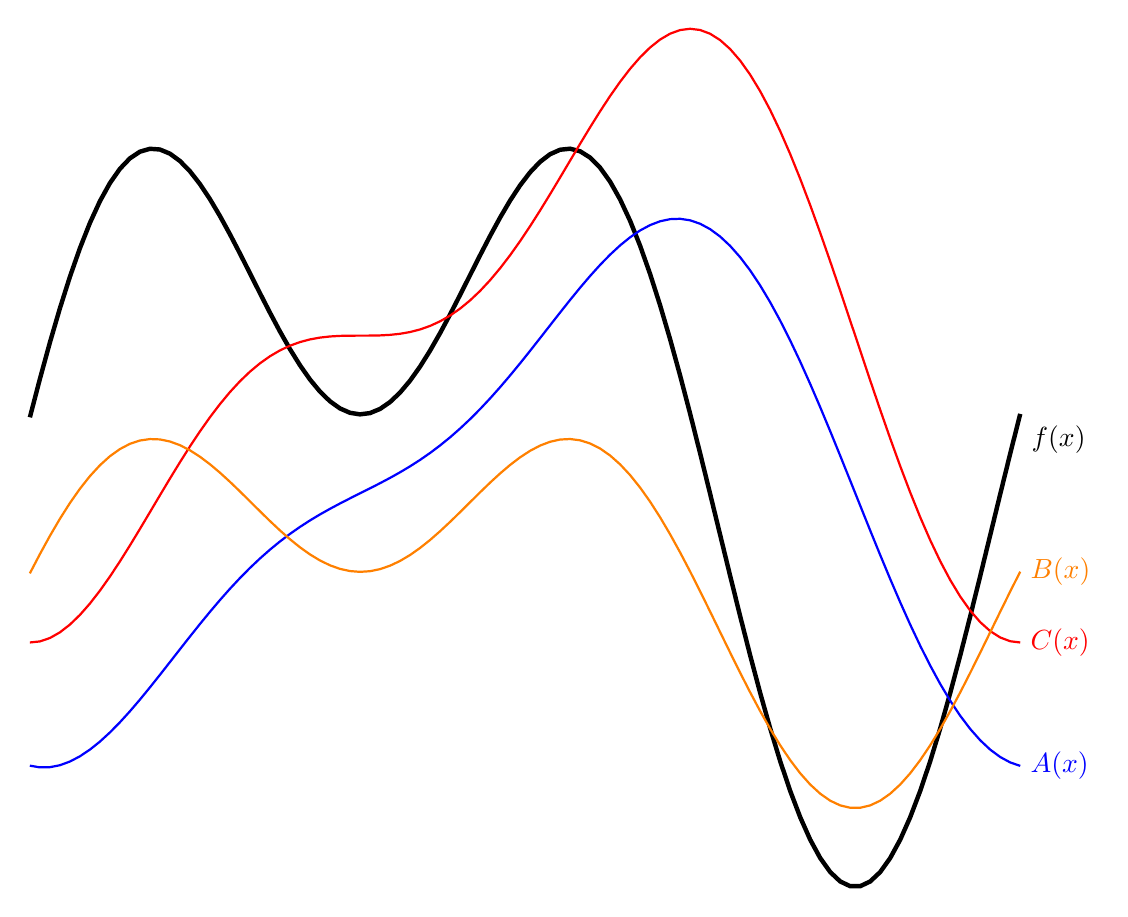
\begin{tikzpicture}
\YEaaxis{8}{6}{6}{6}
\draw[ultra thick] plot[domain=-3.67:2.62, samples=100](2*\x,{3*cos(2*\x r)-3*sin(\x r)}) node[below right]{$f(x)$};%f(x)
\draw[thick, red] plot[domain=-3.67:2.62, samples=100](2*\x,{3*cos(\x r)+1.5*sin(2*\x r)+1}) node[right]{$C(x)$};%F(x)
\draw[thick, blue] plot[domain=-3.67:2.62, samples=100](2*\x,{3*cos(\x r)+sin(2*\x r)-1}) node[right]{$A(x)$};%not
\draw[thick, orange] plot[domain=-3.67:2.62, samples=100](2*\x,{1.5*cos(2*\x r)-1.5*sin(\x r)-2}) node[right]{$B(x)$};%not
\end{tikzpicture}\end{center}
\end{Mquestion}
\begin{hint}
When $f(x)$ is positive, its antiderivative $F(x)$ is increasing. When $f(x)$ is negative, its antiderivative $F(x)$ is decreasing. When $f(x)=0$, $F(x)$ has a horizontal tangent line.
\end{hint}
\begin{answer}
\textcolor{red}{$C(x)$}
\end{answer}
\begin{solution}
Notice $f(x)$ is nonnegative for an interval covering the left part of the graph, and negative on the right part of the graph. That means its antiderivative is increasing for the left interval, then decreasing for the right interval. This applies to $A(x)$ and $C(x)$, but not $B(x)$.

There are only three points where $A(x)$ has a horizontal tangent line: at its global maximum and the endpoints of the interval shown. By contrast, $C(x)$ has a horizontal tangent line in four places: at its global maximum,  at its inflection point, and at the endpoints of the interval shown. Since $f(x)=0$ four times (and these line up with the horizontal portions of $C(x)$) we conclude  $C(x)$ is the antiderivative of $f(x)$.
\end{solution}



%%%%%%%%%%%%%%%%%%
\subsection*{\Procedural}
%%%%%%%%%%%%%%%%%%
\Instructions{In Questions~\ref{s4.1antifirst} through \ref{s4.1antilast}, you are asked to find the antiderivative of a function. Phrased like this, we mean the \emph{most general} antiderivative. These will all include some added constant. The table after Example~\ref*{eg antidiff poly} %4.1.3
might be of help.}

\begin{Mquestion}\label{s4.1antifirst}
Find the  antiderivative of
$f(x)=3x^2+5x^4+10x-9$.
\end{Mquestion}
\begin{hint}
For any constant $n \neq -1$, an antiderivative of $x^n$ is $\frac{1}{n+1}x^{n+1}$.
\end{hint}
\begin{answer}
$F(x)=x^3+x^5+5x^2-9x+C$
\end{answer}
\begin{solution}
For any constant $n \neq -1$, an antiderivative of $x^n$ is $\frac{1}{n+1}x^{n+1}$.
\begin{align*}
F'(x)&=3x^2+5x^4+10x-9\\
F(x)&=3\left(\frac{1}{3}\right)x^3+5\left(\frac{1}{5}\right)x^5+10\left(\frac{1}{2}\right)x^2-9\left(\frac{1}{1}\right)x^1+C\\
&=x^3+x^5+5x^2-9x+C
\end{align*}

Remark: we can always check by differentiating:
\begin{align*}
F'(x)&=\diff{}{x}\left\{x^3+x^5+5x^2-9x+C\right\}\\
&=3x^2+5x^4+10x-9\\
&=f(x)
\end{align*}
so  $F(x)$ is indeed an antiderivative of $f(x)$.
\end{solution}


\begin{question}
Find the  antiderivative of
$f(x)=\dfrac{3}{5}x^7-18x^4+x$.
\end{question}
\begin{hint}
For any constant $n \neq -1$, an antiderivative of $x^n$ is $\frac{1}{n+1}x^{n+1}$.
\end{hint}
\begin{answer}
$F(x)=\dfrac{3}{40}x^8-\dfrac{18}{5}x^5+\dfrac{1}{2}x^2+C$
\end{answer}
\begin{solution}
\begin{align*}
F'(x)&=\frac{3}{5}x^7-18x^4+x\\
F(x)&=\left(\frac{3}{5}\right)\left(\frac{1}{8}\right)x^8-18\left(\frac{1}{5}\right)x^5+\frac{1}{2}x^2+C\\
&=\frac{3}{40}x^8-\frac{18}{5}x^5+\frac{1}{2}x^2+C
\end{align*}
\end{solution}


\begin{Mquestion}
Find the antiderivative of
$f(x)=4\sqrt[3]{x}-\dfrac{9}{2x^{2.7}}$.
\end{Mquestion}
\begin{hint}
For any constant $n\neq -1$, an antiderivative of $x^n$ is $\frac{1}{n+1}x^{n+1}$. The constant $n$ does not have to be an integer.
\end{hint}
\begin{answer}
$F(x)=3x^{\tfrac{4}{3}}+\dfrac{45}{17x^{1.7}}+C$
\end{answer}
\begin{solution}
For any constant $n\ne 1$, an antiderivative of $x^n$ is $\frac{1}{n+1}x^{n+1}$. The constant $n$ does not have to be an integer.
\begin{align*}
F'(x)&=4\sqrt[3]{x}-\frac{9}{2x^{2.7}}\\
&=4 x^{\tfrac{1}{3}}-\frac{9}{2}x^{-2.7}\\
F(x)&=4\left(\frac{1}{\frac{1}{3}+1}\right)x^{\left(\tfrac{1}{3}+1\right)}-\left(\frac{9}{2}\right)\left(\frac{1}{-2.7+1}\right)x^{(-2.7+1)}+C\\
&=4\left(\frac{3}{4}\right)x^{\tfrac{4}{3}}-\left(\frac{9}{2}\right)\left(\frac{10}{-17}\right)x^{-1.7}+C\\
&=3x^{\tfrac{4}{3}}+\frac{45}{17x^{1.7}}+C
\end{align*}
\end{solution}



\begin{question}
Find the  antiderivative of
$f(x)=\dfrac{1}{7\sqrt{x}}$.
\end{question}
\begin{hint}
What is the derivative of $\sqrt{x}$?
\end{hint}
\begin{answer}
$F(x)=\dfrac{2}{7}\sqrt{x}+C$
\end{answer}
\begin{solution}
\begin{itemize}
\item Solution 1:
We can re-write $f(x)$ to make it a power of $x$.
\begin{align*}
F'(x)&=\frac{1}{7}x^{-\tfrac{1}{2}}\\
F(x)&=\left(\frac{1}{7}\right)\left(\frac{1}{-\frac{1}{2}+1}\right)x^{\left(-\tfrac{1}{2}+1\right)}+C\\
&=\left(\frac{1}{7}\right)(2)x^{\tfrac{1}{2}}+C\\
&=\frac{2}{7}\sqrt{x}+C
\end{align*}
\item Solution 2:
We notice that $\dfrac{1}{7\sqrt{x}}$ looks a lot like $\dfrac{1}{2\sqrt{x}}$, which is the derivative of $\sqrt{x}$. So:
\begin{align*}
\diff{}{x}\left\{\sqrt{x}\right\}&=\frac{1}{2\sqrt{x}}\\
\diff{}{x}\left\{\frac{2}{7}\sqrt{x}\right\}&=\left(\frac{2}{7}\right)\frac{1}{2\sqrt{x}}=f(x)
\end{align*}
So, an antiderivative of $f(x)$ is $\dfrac{2}{7}\sqrt{x}$. Then the most general antiderivative is $F(x)=\dfrac{2}{7}\sqrt{x}+C$.
\end{itemize}
\end{solution}


\begin{question}
Find the antiderivative of
$f(x)=e^{5x+11}$.
\end{question}
\begin{hint}
The derivative of $e^{5x+11}$ is close to, but not exactly the same as, $f(x)$.
Don't be afraid to just make a guess. But be sure
          to check by differentiating your guess. If the derivative
          isn't what you want, you will often still learn enough
          to be able to then guess the correct antiderivative.
\end{hint}
\begin{answer}
$F(x)=\dfrac{1}{5}e^{5x+11}+C$
\end{answer}
\begin{solution}
We recall $\ds\diff{}{x}e^x=e^x$. That is, $e^x$ is its own antiderivative.
 So, a first guess for the antiderivative of $f(x)$ might be itself.
 \begin{align*}
 \diff{}{x}\left\{e^{5x+11}\right\}&=5e^{5x+11}
 \intertext{This isn't exactly right, so we modify it by multiplying by a constant.}
 \diff{}{x}\left\{\frac{1}{5}e^{5x+11}\right\}&=e^{5x+11}
  \end{align*}
  This tells us that $\dfrac{1}{5}e^{5x+11}$ is an antiderivative of $e^{5x+11}$. Therefore, the most general antiderivative of $e^{5x+11}$ is $F(x)=\dfrac{1}{5}e^{5x+11}+C$.
\end{solution}



\begin{Mquestion}
Find the antiderivative of
$f(x)=3\sin(5x)+7\cos(13x)$.
\end{Mquestion}
\begin{hint}
From the table in the text, an antiderivative of $\sin x$ is $-\cos x$, and an antiderivative of $\cos x$ is $\sin x$.
\end{hint}
\begin{answer}
$F(x)=-\dfrac{3}{5}\cos(5x)+\dfrac{7}{13}\sin(13x)+C$
\end{answer}
\begin{solution}
We know the derivatives of sine and cosine. We'll work from there to build a function whose derivative is $f(x)$. We'll start by finding an antiderivative of $7\cos(13x)$.
\begin{align*}
\diff{}{x}\{\sin x\}&=\cos x\\
\diff{}{x}\{\sin(13x)\}&=13\cos(13x)\\
\diff{}{x}\left\{\frac{1}{13}\sin(13x)\right\}&=\frac{13}{13}\cos(13x)=\cos(13x)\\
\diff{}{x}\left\{\frac{7}{13}\sin(13x)\right\}&=7\cos(13x)
\intertext{So, an antiderivative of $7\cos(13x)$ is $\dfrac{7}{13}\sin(13x)$.}
\diff{}{x}\{\cos x\}&=-\sin x\\
\diff{}{x}\{-\cos x\}&=\sin x\\
\diff{}{x}\{-\cos (5x)\}&=5\sin (5x)\\
\diff{}{x}\left\{-\frac{3}{5}\cos (5x)\right\}&=\left(\frac{3}{5}\right)5\sin (5x)=3\sin(5x)\\
\end{align*}
So, an antiderivative of $3\sin(5x)$ is $-\dfrac{3}{5}\cos(5x)$.

The most general antiderivative of $3\sin(5x)+7\cos(13x)$ is\\
$F(x)=-\dfrac{3}{5}\cos(5x)+\dfrac{7}{13}\sin(13x)+C$.
\end{solution}

\begin{question}
Find the antiderivative of
$f(x)=\sec^2(x+1)$.
\end{question}
\begin{hint}
What is the derivative of tangent?
\end{hint}
\begin{answer}
$F(x)=\tan(x+1)+C$
\end{answer}
\begin{solution}
We know the derivative of $\tan x$ is $\sec^2 x$. Modifying this slightly, we see (using the chain rule)
\begin{align*}
\diff{}{x}\left\{\tan(x+1)\right\}&=\sec^2(x+1)\cdot\diff{}{x}\{x+1\}\\
&=\sec^2(x+1)
\end{align*}
So, $\tan(x+1)$ is an antiderivative of $\sec^2(x+1)$. Therefore, the most general antiderivative of $\sec^2(x+1)$ is
$F(x)=\tan(x+1)+C$.
\end{solution}


\begin{Mquestion}
Find the antiderivative of
$f(x)=\dfrac{1}{x+2}$.
\end{Mquestion}
\begin{hint}
What is an antiderivative of $\dfrac{1}{x}$?
\end{hint}
\begin{answer}
$F(x)=\log|x+2|+C$
\end{answer}
\begin{solution}
We note that $f(x)$ looks similar to $\dfrac{1}{x}$.
\begin{align*}
\diff{}{x}\left\{\log|x|\right\}&=\frac{1}{x}\\
\diff{}{x}\left\{\log|x+2|\right\}&=\frac{1}{x+2}
\end{align*}
The most general antiderivative of $f(x)$ is $F(x)=\log|x+2|+C$.
\end{solution}

\begin{question}\label{s4.1arcsin1}
Find the antiderivative of
$f(x)=\dfrac{7}{\sqrt{3-3x^2}}$.
\end{question}
\begin{hint}
$\dfrac{7}{\sqrt{3-3x^2}}=\dfrac{7}{\sqrt{3}}\left(\dfrac{1}{\sqrt{1-x^2}}\right)$
\end{hint}
\begin{answer}
$F(x)=\dfrac{7}{\sqrt{3}}\arcsin(x)+C$
\end{answer}
\begin{solution}
Our function $f(x)$ bears some resemblance to the derivative of arcsine, $\dfrac{1}{\sqrt{1-x^2}}$:
\begin{align*}
f(x)=\dfrac{7}{\sqrt{3-3x^2}}&=\dfrac{7}{\sqrt{3}}\left(\dfrac{1}{\sqrt{1-x^2}}\right)\\
\diff{}{x}\left\{\frac{7}{\sqrt{3}}\arcsin(x)\right\}&=\frac{7}{\sqrt{3}}\left(\frac{1}{\sqrt{1-x^2}}\right)=f(x)
\end{align*}
So, the most general antiderivative of $f(x)$ is
$F(x)=\dfrac{7}{\sqrt{3}}\arcsin(x)+C$.
\end{solution}



\begin{Mquestion}\label{s4.1antilast}
Find the antiderivative of
$f(x)=\dfrac{1}{1+25x^2}$
\end{Mquestion}
\begin{hint}
How is this similar to the derivative of the arctangent function?
\end{hint}
\begin{answer}
$F(x)=\dfrac{1}{5}\arctan(5x)+C$
\end{answer}
\begin{solution}
We notice that $f(x)$ looks similar to the derivative of the arctangent function, $\dfrac{1}{1+x^2}$.
\begin{align*}
f(x)=\frac{1}{1+25x^2}&=\frac{1}{1+(5x)^2}
\intertext{This gives us a first guess for our antiderivative: perhaps $\arctan(5x)$ will work. We test it by differentiating, making sure we don't forget the chain rule.}
\diff{}{x}\left\{\arctan(\textcolor{red}{5x})\right\}&=\frac{1}{1+\left(\textcolor{red}{5x}\right)^2}\cdot\textcolor{red}{5}
\intertext{We're close to $f(x)$, but we've multiplied by 5. That's easy to take care of: we can divide our guess by 5.}
\diff{}{x}\left\{\frac{1}{5}\arctan(\textcolor{red}{5x})\right\}&=
\frac{1}{5}\left(\frac{1}{1+\left(\textcolor{red}{5x}\right)^2}\right)\cdot\textcolor{red}{5}\\
&=\frac{1}{1+25x^2}=f(x)
\end{align*}
So, the most general antiderivative of $f(x)$ is $F(x)=\dfrac{1}{5}\arctan(5x)+C$.
\end{solution}

\Instructions{In Questions~\ref{s4.1initfirst} through \ref{s4.1initlast}, you are asked to find a specific antiderivative of a function. In this case, you should be able to solve for the entire function--no unknown constants floating about.}


\begin{Mquestion}\label{s4.1initfirst}
Find the function $f(x)$ with $f'(x)=3x^2-9x+4$ and $f(1)=10$.
\end{Mquestion}
\begin{hint}
First, find the antiderivative of $f'(x)$. Your answer will have an unknown $+C$ in it. Figure out which value of $C$ gives $f(1)=10$.
\end{hint}
\begin{answer}
$f(x)=x^3-\dfrac{9}{2}x^2+4x+\dfrac{19}{2}$
\end{answer}
\begin{solution}
First, let's find the antiderivative of $f'(x)$. It's a polynomial, so we can use the observation from the text that an antiderivative of $x^n$, for any constant $n\ne 1$, is
$\frac{1}{n+1}x^{n+1}$. Remember that the most general antiderivative will have an added constant.
\begin{align*}
f(x)&=\frac{3}{3}x^3-\frac{9}{2}x^2+4x+C\\
&=x^3-\frac{9}{2}x^2+4x+C
\intertext{Use the fact that $f(1)=10$ to solve for $C$.}
10&=1-\frac{9}{2}+4+C\\
C&=\frac{19}{2}
\intertext{All together,}
f(x)&=x^3-\frac{9}{2}x^2+4x+\frac{19}{2}.
\end{align*}
\end{solution}


\begin{Mquestion}
Find the function $f(x)$ with $f'(x)=\cos(2x)$ and $f(\pi)=\pi$.
\end{Mquestion}
\begin{hint}
Remember that one antiderivative of $\cos x$ is  $\sin x$ (not ~~$-\sin x$).
\end{hint}
\begin{answer}
$f(x)=\dfrac{1}{2}\sin(2x)+\pi$
\end{answer}
\begin{solution}
First, let's find the antiderivative of $f'(x)$. We know that one antiderivative of $\cos(x)$ is $\sin x$. We might guess that an antiderivative of $\cos(2x)$ is $\sin(2x)$. Check by differentiating:
\begin{align*}
\diff{}{x}\left\{\sin(2x)\right\}&=2\cos(2x)
\intertext{This is close to $f'(x)$, but we need to divide by 2.}
\diff{}{x}\left\{\frac{1}{2}\sin(2x)\right\}&=\cos(2x)
\intertext{So, $f(x)=\dfrac{1}{2}\sin(2x)+C$ for some constant $C$. We can find $C$ using the given information $f(\pi)=\pi$.}
\pi=f(\pi)&=\frac{1}{2}\sin(2\pi)+C\\
\pi&=C
\end{align*}
Therefore, $f(x)=\dfrac{1}{2}\sin(2x)+\pi$.
\end{solution}



\begin{question}
Find the function $f(x)$ with $f'(x)=\dfrac{1}{x}$ and $f(-1)=0$.
\end{question}
\begin{hint}
An antiderivative of $\dfrac{1}{x}$ is $\log(x)+C$, but this is not the most general antiderivative.
\end{hint}
\begin{answer}
$f(x)=\log|x|$
\end{answer}
\begin{solution}
Looking at the table in the notes, we see the antiderivative of $\dfrac{1}{x}$ is $f(x)=\log|x|+C$. The given information $f(-1)=0$ lets us find $C$:
\begin{align*}
0=f(-1)&=\log|-1|+C\\
0&=\log(1)+C\\
0&=C
\end{align*}
So, $f(x)=\log|x|$.

Remark: it is true that $\log x$ is an antiderivative of $\dfrac{1}{x}$, since the derivative of $\log x$ is $\dfrac{1}{x}$. However, $\log x$ is only defined for positive values of $x$. Since the given information tells you that $f(x)$ is defined when $x=-1$, you need to use a more general antiderivative of $\dfrac{1}{x}$: $\log|x|+C$.
\end{solution}


\begin{question}\label{s4.1initlast}
Find the function $f(x)$ with $f'(x)=\dfrac{1}{\sqrt{1-x^2}}+1$ and $f(1)=-\dfrac{\pi}{2}$.
\end{question}
\begin{hint}
What is the derivative of the arcsine function?
\end{hint}
\begin{answer}
$f(x)=\arcsin x+x - \pi-1$
\end{answer}
\begin{solution}
An antiderivative of  $1$ is $x$, and an antiderivative of $\dfrac{1}{\sqrt{1-x^2}}$ is $\arcsin(x)$. So, $f(x)=\arcsin x + x +C$. The given information lets us find $C$.
\begin{align*}
-\frac{\pi}{2}=f(1)&=\arcsin(1)+1+C\\
-\frac{\pi}{2}&=\frac{\pi}{2}+1+C\\
C&=-\pi-1
\end{align*}
So, $f(x)=\arcsin x+x - \pi-1$.
\end{solution}

\Instructions{In Questions~\ref{s4.1applyfirst} through \ref{s4.1applylast}, we will explore some simple situations where antiderivatives might arise.}


\begin{Mquestion}\label{s4.1applyfirst}
Suppose a population of bacteria at time $t$ (measured in hours) is growing at a rate of $100e^{2t}$ individuals per hour. Starting at time $t=0$, how long will it take the initial colony to increase by 300 individuals?
\end{Mquestion}
\begin{hint}
If $P(t)$ is the population at time $t$, then the information given in the problem is
$P'(t)=100e^{2t}$.
\end{hint}
\begin{answer}
It takes $\frac{1}{2}\log 7$ hours (about 58 minutes) for the initial colony to increase by 300 individuals.
\end{answer}
\begin{solution}
If $P(t)$ is the population at time $t$, then the information given in the problem is
$P'(t)=100e^{2t}$. Antidifferentiating, we see $P(t)=50e^{2t}+C$, where $C$ is some constant. We want to know for what value of $t$ we get $P(t)=P(0)+300$.
\begin{align*}
P(t)&=P(0)+300\\
50e^{2t}+C&=50e^{0}+C+300\\
50e^{2t}&=350\\
e^{2t}&=7\\
2t&=\log(7 )\\
t&=\frac{1}{2}\log(7)
\end{align*}
It takes $\frac{1}{2}\log 7$ hours (about 58 minutes) for the initial colony to increase by 300 individuals.
\end{solution}



\begin{question}
Your bank account at time $t$ (measured in years) is growing at a rate of
\[1500e^{\tfrac{t}{50}} \]
dollars per year. How much money is in your account at time $t$?
\end{question}
\begin{hint}
You can't know exactly--there will be a constant involved.
\end{hint}
\begin{answer}
At time $t$, the amount of money in your bank account is $75000e^{\tfrac{t}{50}}+C$ dollars, for some constant $C$.
\end{answer}
\begin{solution}
If $A(t)$ is the amount of money in your account at time $t$, then the given information is
\begin{align*}
A'(t)&=1500e^{\tfrac{t}{50}}
\intertext{Antidifferentiating,}
A(t)&=75000e^{\tfrac{t}{50}}+C
\intertext{for some constant $C$.}
\end{align*}
That is, at time $t$, the amount of money in your bank account is $75000e^{\tfrac{t}{50}}+C$ dollars, for some constant $C$.
\end{solution}



\begin{question}\label{s4.1applylast}
At time $t$ during a particular day, $0 \leq t \leq 24$, your house consumes energy at a rate of \[0.5\sin\left(\frac{\pi}{24}t\right)+0.25\] kW. (Your consumption was smallest in the middle of the night, and peaked at noon.) How much energy did your house consume in that day?
\end{question}
\begin{hint}
If $P(t)$ is the amount of power in kW-hours the house has used since time $t=0$, where $t$ is measured in hours, then the information given is that $P'(t)=0.5\sin\left(\dfrac{\pi}{24}t\right)+0.25$ kW.
\end{hint}
\begin{answer}
$\dfrac{24}{\pi}+6\approx13.6$ kWh
\end{answer}
\begin{solution}
Let $P(t)$ be the amount of power your house has used since time $t=0$. If $t$ is measured in hours, and $P(t)$ in kWh (kilowatt-hours), then $P'(t)$ is the rate at which your house is consuming power, in kW. So, the given information is that
\begin{align*}
P'(t)&=0.5\sin\left(\dfrac{\pi}{24}t\right)+0.25
\intertext{Antidifferentiating,}
P(t)&=-\frac{12}{\pi}\cos\left(\frac{\pi}{24}t\right)+0.25t+C
\intertext{Since $P(0)$ is the amount of energy consumed after 0 hours, $P(0)=0$, so}
0=P(0)&=-\frac{12}{\pi}+C\\
C&=\frac{12}{\pi}\\
P(t)&=\frac{12}{\pi}\left[1-\cos\left(\frac{\pi}{24}t\right)\right]+0.25t
\intertext{After 24 hours, your energy consumed is}
P(24)&=\frac{12}{\pi}\left[1-\cos\left(\pi\right)\right]+0.25(24)\\
&=\frac{24}{\pi}+6\approx13.6~ \mathrm{kWh}
\end{align*}
\end{solution}



%%%%%%%%%%%%%%%%%%
\subsection*{\Application}
%%%%%%%%%%%%%%%%%%


\begin{question}[1999H]
Let $f(x)=2\sin^{-1}\sqrt{x}$ and $g(x)=\sin^{-1}(2x-1)$.
Find the derivative of $f(x)-g(x)$ and simplify your answer. What does
the answer imply about the relation between $f(x)$ and $g(x)$?
\end{question}
\begin{hint}
The derivatives should match. Remember $\sin^{-1}$ is another way of writing arcsine.
\end{hint}
\begin{answer}
$f'(x)=g'(x)=\dfrac{1}{\sqrt{x-x^2}}$; $f$ and $g$ differ only by a constant.
\end{answer}
\begin{solution}
We differentiate $f(x)$ and $g(x)$ using the chain rule. Recall $\ds\diff{}{x}\left\{\arcsin(x)\right\}=\dfrac{1}{\sqrt{1-x^2}}$.
\begin{align*}
f'(x)&=\frac{2}{\sqrt{1-\textcolor{red}{\sqrt{x}}^2}}\cdot\diff{}{x}\textcolor{red}{\sqrt{x}}\\
&=\frac{2}{\sqrt{1-x}}\cdot\frac{1}{2\sqrt{x}}\\
&=\frac{1}{\sqrt{x-x^2}}\cr
g'(x)&=\frac{1}{\sqrt{1-\textcolor{red}{(2x-1)}^2}}\cdot\diff{}{x}\{\textcolor{red}{2x-1}\}\\
&=\frac{2}{\sqrt{1-4x^2+4x-1}}\\
&=\frac{1}{\sqrt{x-x^2}}\cr
\end{align*}
So, the derivative of $f(x)-g(x)$ is $0$, which implies that
$f(x)$ and $g(x)$ differ by a constant--perhaps a surprising result!

Remark: we don't need calculus to show that $f(x)$ and $g(x)$ only differ by a constant. Define
$\theta=\sin^{-1}\sqrt{x}$, so that $\sin\theta=\sqrt{x}$ and $f(x) = 2\theta$ , and then
$$
\sin \left[f(x)-\frac{\pi}{2}\right]=-\cos f(x) =-\cos 2\theta=-[1-2\sin^2\theta]
=2\sin^2\theta -1=2x-1
$$
Our goal is to take the arcsine of the first and last expressions and conclude $f(x)-\dfrac{\pi}{2}=\arcsin(2x-1)=g(x)$. However, before we can say $\arcsin\left(\sin\left[f(x)-\dfrac{\pi}{2}\right]\right)=f(x)-\dfrac{\pi}{2}$, we have to check that $-\dfrac{\pi}{2} \leq f(x)-\dfrac{\pi}{2}\leq\dfrac{\pi}{2}$. That is, we need to show that $0 \leq f(x) \leq \pi$.

%Since~~ $\sin g(x)=2x-1$, we have that $\sin\big(f(x)-\frac{\pi}{2}\big)=\sin g(x)$.
 As  $0\le\theta\le\frac{\pi}{2}$
(since $\sin^{-1}$ always takes values between
$-\frac{\pi}{2}$ and $\frac{\pi}{2}$ and since $\sqrt{x}\ge 0$),
we have that $0\le f(x)=2\theta\le \pi$. So,
\[f(x)-\dfrac{\pi}{2}=\arcsin\left(\sin\left[f(x)-\dfrac{\pi}{2}\right]\right)=\arcsin(2x+1)=g(x).\]
\end{solution}



\Instructions{For Questions~\ref{s4.1rulesfirst} through \ref{s4.1ruleslast}, you are again asked to find the  antiderivatives of certain functions. In general, finding antiderivatives can be extremely difficult--indeed, it will form the main topic of next semester's calculus course. However, you can work out the antiderivatives of the functions below using what you've learned so far about derivatives.}

\begin{question}\label{s4.1rulesfirst}
Find the  antiderivative of $f(x)=2\cos(2x)\cos(3x)-3\sin(2x)\sin(3x)$.
\end{question}
\begin{hint}
Think about the product rule.
\end{hint}
\begin{answer}
$F(x)=\sin(2x)\cos(3x)+C$
\end{answer}
\begin{solution}
The derivative of $\sin(2x)$ (which occurs in the second term) is $2\cos(2x)$ (which occurs in the first term). Similarly, the derivative of $\cos(3x)$ (which occurs in the first term) is $-3\sin(3x)$ (which occurs in the second term). So, $f(x)$ seems to have come from the product rule.
\[\diff{}{x}\{\sin(2x)\cos(3x)\}=2\cos(2x)\cos(3x)-3\sin(2x)\sin(3x)\]
Then the antiderivative of $f(x)$ is $F(x)=\sin(2x)\cos(3x)+C$.
\end{solution}




\begin{question}
Find the  antiderivative of $f(x)=\dfrac{(x^2+1)e^x-e^x(2x)}{(x^2+1)^2}$.
\end{question}
\begin{hint}
Think about the quotient rule for derivatives.
\end{hint}
\begin{answer}
$F(x)=\dfrac{e^x}{x^2+1}+C$
\end{answer}
\begin{solution}
The function $f(x)$ looks like perhaps it came from the quotient rule. Recall
\begin{align*}
\diff{}{x}\left\{\frac{\textcolor{red}{u(x)}}{\textcolor{blue}{v(x)}}\right\}&=
\frac{\textcolor{blue}{v(x)}\textcolor{red}{u'(x)}-\textcolor{red}{u(x)}\textcolor{blue}{v'(x)}}{(\textcolor{blue}{v(x)})^2}
\intertext{Then, since the denominator of $f(x)$ is $(x^2+1)^2$, we might guess $v(x)=(x^2+1)$. That leaves $u(x)=e^x$.}
\diff{}{x}\left\{\frac{e^x}{x^2+1}\right\}&=\frac{(x^2+1)e^x-e^x(2x)}{(x^2+1)^2}=f(x)
\end{align*}
So, the antiderivative of $f(x)$ is $F(x)=\dfrac{e^x}{x^2+1}+C$.
\end{solution}



\begin{Mquestion}\label{s4.1chain}
Find the antiderivative of
$f(x)=3x^2e^{x^3}$.
\end{Mquestion}
\begin{hint}
Notice that the derivative of $x^3$  is $3x^2$.
\end{hint}
\begin{answer}
$F(x)=e^{x^3}+C$
\end{answer}
\begin{solution}
We know that $e^x$ is its own antiderivative. The derivative of $e^{g(x)}$, for some function $g(x)$, is $g'(x)e^{g(x)}$. Since $3x^2$ is the derivative of $x^3$, $f(x)$ fits this pattern. We guess
the antiderivative of $f(x)$ is $F(x)=e^{x^3}+C$.

We check by differentiating.
\begin{align*}
\diff{}{x}\left\{e^{x^3}+C\right\}&=3x^2e^{x^3}=f(x)
\end{align*}

Indeed, the antiderivative of $f(x)$ is $F(x)=e^{x^3}+C$.
\end{solution}



\begin{question}
Find the  antiderivative of
$f(x)=5x\sin(x^2)$.
\end{question}
\begin{hint}
Think about the chain rule for derivatives. You might need to multiply your first guess by a constant.
\end{hint}
\begin{answer}
$F(x)=-\dfrac{5}{2}\cos(x^2)+C$
\end{answer}
\begin{solution}
We know the antiderivative of $\sin x$ is $-\cos x $. Since  $\sin(x^2)$ appears in our function, let's investigate the derivative of $-\cos(x^2)$.
\begin{align*}
\diff{}{x}\left\{-\cos\left(x^2\right)\right\}&=\sin\left(x^2\right)\cdot2x
\intertext{This differs from $f(x)$ only by a constant multiple.}
\diff{}{x}\left\{-\frac{5}{2}\cos\left(x^2\right)\right\}&=\frac{5}{2}\sin\left(x^2\right)\cdot2x=5x\sin(x^2)=f(x)
\end{align*}
So, the antiderivative of $f(x)$ is $F(x)=-\dfrac{5}{2}\cos\left(x^2\right)+C$

Remark: as in Question~\ref{s4.1chain},  our function $f(x)$ involved some function $g(x)$ as well as $g'(x)$. This pattern is the basis of an important method of antidifferentiation, called the Substitution Rule.
\end{solution}




\begin{question}
Find the  antiderivative of
$f(x)=e^{\log x}$.
\end{question}
\begin{hint}
Simplify.
\end{hint}
\begin{answer}
$F(x)=\dfrac{1}{2}x^2+C$.
\end{answer}
\begin{solution}
For any $x$ in the domain of $\log (x)$, $e^{\log x}=x$. So, $f(x)=x$ for every $x$ in its domain. Then its antiderivative is $F(x)=\dfrac{1}{2}x^2+C$.
\end{solution}


\begin{Mquestion}\label{s4.1ruleslast}
Find the antiderivative of
$f(x)=\dfrac{7}{\sqrt{3-x^2}}$.
\end{Mquestion}
\begin{hint}
This problem is similar to Question~\ref{s4.1arcsin1}, but you'll have to do some harder factoring. Try getting $f(x)$ into the form $a\left(\dfrac{1}{\sqrt{1-(bx)^2}}\right)$ for some constants $a$ and $b$.
\end{hint}
\begin{answer}
$F(x)=7\arcsin\left(\dfrac{x}{\sqrt{3}}\right)+C$
\end{answer}
\begin{solution}
As in  Question~\ref{s4.1arcsin1}, we notice that our function is similar to $\dfrac{1}{\sqrt{1-x^2}}$, but in this case it doesn't factor quite as nicely.
\begin{align*}
f(x)=\frac{7}{\sqrt{3-x^2}}&=\frac{7}{\sqrt{3(1-\frac{x^2}{3})}}
\\&=\frac{7}{\sqrt{3}}\left(\frac{1}{\sqrt{1-\frac{x^2}{3}}}\right)
\intertext{What we really want under that square root, instead of $\dfrac{x^2}{3}$, is simply  $x^2$. We can get close: we can get \emph{something} squared.}
f(x)&=\frac{7}{\sqrt{3}}\left(\frac{1}{\sqrt{1-\left(\frac{x}{\sqrt{3}}\right)^2}}\right)
\intertext{Now, the thing that's squared isn't $x$, it's $\dfrac{x}{\sqrt{3}}$. This gives us a first guess for an antiderivative: perhaps $F(x)=\dfrac{7}{\sqrt{3}}\arcsin\left(\dfrac{x}{\sqrt{3}}\right)$ will work. Let's try it! Remember to use the chain rule when you differentiate.}
\diff{}{x}\left\{\frac{7}{\sqrt{3}}\arcsin\left(\textcolor{red}{\frac{x}{\sqrt{3}}}\right)\right\}&=
\frac{7}{\sqrt{3}}\left(\frac{1}{\sqrt{1-\left(\textcolor{red}{\frac{x}{\sqrt{3}}}\right)^2}}\right)\cdot\textcolor{red}{\frac{1}{\sqrt{3}}}
\intertext{We're very close! We're only off by a constant, and those are easy to fix. We're dividing by $\sqrt{3}$ when we differentiate, so let's multiply our function by $\sqrt{3}$.}
\diff{}{x}\left\{7\arcsin\left(\textcolor{red}{\frac{x}{\sqrt{3}}}\right)\right\}&=
7\left(\frac{1}{\sqrt{1-\left(\textcolor{red}{\frac{x}{\sqrt{3}}}\right)^2}}\right)\cdot\textcolor{red}{\frac{1}{\sqrt{3}}}\\
&=\frac{7}{\sqrt{3}\sqrt{1-\left(\frac{x}{\sqrt{3}}\right)^2}}\\
&=\frac{7}{\sqrt{3-x^2}}=f(x)
\end{align*}
Therefore, the most general antiderivative of $f(x)$ is
$F(x)=7\arcsin\left(\dfrac{x}{\sqrt{3}}\right)+C$.
\end{solution}



\begin{question}
Imagine forming a solid by revolving the parabola $y=x^2+1$ around the $x$-axis, as in the picture below.
\begin{center}
\begin{tikzpicture}
\draw[->, red] (-4,.25) arc(40:340:.15 cm and .5 cm);
\draw[thick] (-3,0) node[shape=ellipse, minimum width=1cm, minimum height=4cm, draw, fill=gray!20]{};
\draw[thick] (3,2) arc(90:-90:.5cm and 2cm);
%\draw[loosely dashed] (3,2) arc(90:270:.5cm and 2cm);
\draw[red, thick] plot[domain=-1:1](3*\x,{\x*\x+1}) node[above]{$y=x^2+1$};
\draw[thick] plot[domain=-1:1](3*\x,{-\x*\x-1});
\draw [help lines, ->] (0,-1)-- (0,-3);
\draw [help lines, ->] (0,1)-- (0,3)node[above]{$y$};
%\draw[help lines, dashed] (0,-1)--(0,1) (-3,0)--(3.5,0);
\draw[help lines, ->] (-3,0)--(-5,0);
\draw[help lines, ->] (3.5,0)--(5,0) node[right]{$x$};
\end{tikzpicture}
\end{center}
Use the method of Example~\ref*{eg vol cone} %4.1.7
to find the volume of such an object if the segment of the parabola that we rotate runs from $x=-H$ to $x=H$.
\end{question}
\begin{hint}
Following Example~\ref*{eg vol cone}, %4.1.7
let $V(H)$ be the volume of the solid formed by rotating the segment of the parabola from $x=-H$ to $x=H$.
            The plan is to evaluate\\
              $V'(H) = \ds\lim\limits_{h\rightarrow H}\frac{V(H)-V(h)}{H-h}$
            and then antidifferentiate $V'(H)$ to find $V(H)$. Since
            you don't know $V(H)-V(h)$ (yet), first find upper and lower
            bounds on it when $h<H$. These bounds can be the volumes of
            two cylinders, one with radius $H$ (and what height?)
            and the other with radius $h$.
\end{hint}
\begin{answer}
$V(H)=2\pi\left(\dfrac{1}{5}H^5+\dfrac{2}{3}H^3+H\right)$
\end{answer}
\begin{solution}
Following Example~\ref*{eg vol cone}, %4.1.7
let $V(H)$ be the volume of the solid formed by rotating the segment of the parabola from $x=-H$ to $x=H$. \textcolor{red}{
 Our plan is to evaluate
              $V'(H) = \ds\lim\limits_{h\rightarrow H}\frac{V(H)-V(h)}{H-h}$
            and then antidifferentiate $V'(H)$ to find $V(H)$. Since
            we don't know $V(H)-V(h)$ (yet) we first find upper and lower
            bounds on it when $h<H$.
}

For a constant $h<H$, $V(H)-V(h)$ is the volume of the solid inside the larger object (with length $2H$) and outside the smaller object (with length $2h$, shown below in blue). There are two regions inside the larger object and outside the smaller.
\begin{center}
\begin{tikzpicture}
\draw[thick] (-3,0) node[shape=ellipse, minimum width=1cm, minimum height=4cm, draw, fill=gray!20]{};
\draw[thick] (3,2) arc(90:-90:.5cm and 2cm);
\draw[thick] plot[domain=-1:1](3*\x,{\x*\x+1});% node[above]{$y=x^2+1$};
\draw[thick] plot[domain=-1:1](3*\x,{-\x*\x-1});
%\draw (3,2) node[vertex, label=above right:{$(H,H^2+1)$}]{};
\draw [help lines, ->] (0,-1)-- (0,-2.5);
\draw [help lines, ->] (0,1)-- (0,3)node[above]{$y$};
\draw[help lines, ->] (-3,0)--(-5,0);
\draw[help lines, ->] (3.5,0)--(5,0) node[right]{$x$};
\draw[decorate, decoration={brace, amplitude=10pt, mirror}] (0,-4)--(3,-4);
\draw (1.5,-4.75) node{$H$};
\color{blue}
\draw[ decorate, decoration={brace, amplitude=10pt, mirror}] (0,-3)--(2,-3);
\draw (1,-3.75) node{$h$};
%\draw[thick, fill=blue!10] (2,13/9) arc(90:-90:.33cm and 1.44 cm) .. controls (.33 , -.85) and (-.33,-.85).. (-2,-13/9) arc(-90:90:.33cm and 1.44 cm) .. controls (-.33 , .85) and (.33,.85).. (2,13/9);
\filldraw[draw=blue, bottom color=blue!50!black, top color=cyan] (2,13/9) arc(90:-90:.33cm and 1.44 cm) .. controls (.33 , -.85) and (-.33,-.85).. (-2,-13/9) arc(-90:90:.33cm and 1.44 cm) .. controls (-.33 , .85) and (.33,.85).. (2,13/9);
%\draw[blue] (2,1.44) node[vertex, label=above left:{$(h,h^2+1)$}]{};
\end{tikzpicture}
\end{center}
One of the regions inside the larger object and outside the smaller (blue) object looks like this:
\begin{center}\begin{tikzpicture}
\draw (0,0) node[shape=ellipse, fill=gray!10, draw, minimum width=1cm, minimum height=3cm]{};
\draw (2,2) arc(90:-90:.67cm and 2cm);
\draw[dashed] (2,2) arc(90:270:.67cm and 2cm);
\draw plot[domain=0:3](\x,{\x*\x/8+1.5}) node[right]{$y=x^2+1$};
\draw plot[domain=0:2](\x,{-\x*\x/8-1.5});
\draw[decorate, decoration={brace, mirror, amplitude=10pt}] (0,-2.5)--(2,-2.5);
\draw (1,-3.25) node{$H-h$};
%\draw (0,0) node[vertex]{};
%\draw (0,0)--(0,1.5);
%\draw (0,.75) node[left]{$h^2+1$};
%\draw (2,0)--(2,2);
%\draw (2,1) node[right]{$H^2+1$};
\draw[help lines, <-] (-2,0)--(0,0);
\draw[help lines, ->] (2.67,0)--(4,0) node[right]{$x$};
\draw[help lines, loosely dashed] (0,0)--(2.67,0);
\YExcoord{0}{h}
\color{gray}\YExcoord{2}{H}
\end{tikzpicture}\end{center}
Remember we formed this solid by rotating the curve $y=x^2+1$ about the $x$-axis. So, the cross-section of this solid is a circle, and the radius of the circle when we are $x$ units from the origin is $x^2+1$. So, the largest radius of the little shape shown above, which occurs at the right end, is $H^2+1$, and the smallest radius (at the left end) is $h^2+1$.

The volume of the shape shown above is less than a cylinder of radius $H^2+1$ and height $H-h$, and it is more than the volume of a cylinder of radius $h^2+1$ and height $H-h$. So, the volume of the shape shown above is between $(H-h)\pi(h^2+1)^2$ and $(H-h)\pi(H^2+1)^2$ cubic units.

Recall that the volume inside the object of length $2H$ and outside the object of length $2h$ consists of \emph{two} copies of the shape shown above. Therefore:
\begin{align*}
2(H-h)\pi(h^2+1)^2 &&<&&V(H)-V(h)&&<&&2(H-h)\pi(H^2+1)^2
\intertext{\color{red}Now that we have upper and lower bounds for $V(H)-V(h)$, we can find $V'(H)$.}
\frac{2(H-h)\pi(h^2+1)^2}{H-h} &&<&&\frac{V(H)-V(h)}{H-h}&&<&&\frac{2(H-h)\pi(H^2+1)^2}{H-h}\\
2\pi(h^2+1)^2 &&<&&\frac{V(H)-V(h)}{H-h}&&<&&2\pi(H^2+1)^2\\
\lim_{h \to H}2\pi(h^2+1)^2 &&\le&&\lim_{h \to H}\frac{V(H)-V(h)}{H-h}&&\le&&\lim_{h \to H}2\pi(H^2+1)^2
\end{align*}
Since the limits on both ends are simply $2\pi(H^2+1)^2$, by the Squeeze Theorem,
\[V'(H)=\lim_{h \to H}\frac{V(H)-V(h)}{H-h}=2\pi(H^2+1)^2\]
\textcolor{red}{Now that we know $V'(H)$, we antidifferentiate to find $V(H)$.}
\begin{align*}
V'(H)&=2\pi(H^4+2H^2+1)\\
V(H)&=2\pi\left(\frac{1}{5}H^5+\frac{2}{3}H^3+H\right)+C
\intertext{When $H=0$, there is no solid, so $V(0)=0$. Therefore,}
V(H)&=2\pi\left(\frac{1}{5}H^5+\frac{2}{3}H^3+H\right).
\end{align*}
\end{solution}
